\section{Qualitative Analysis}
\label{app:qualitative}

\begin{figure*}[t]
  \centering
  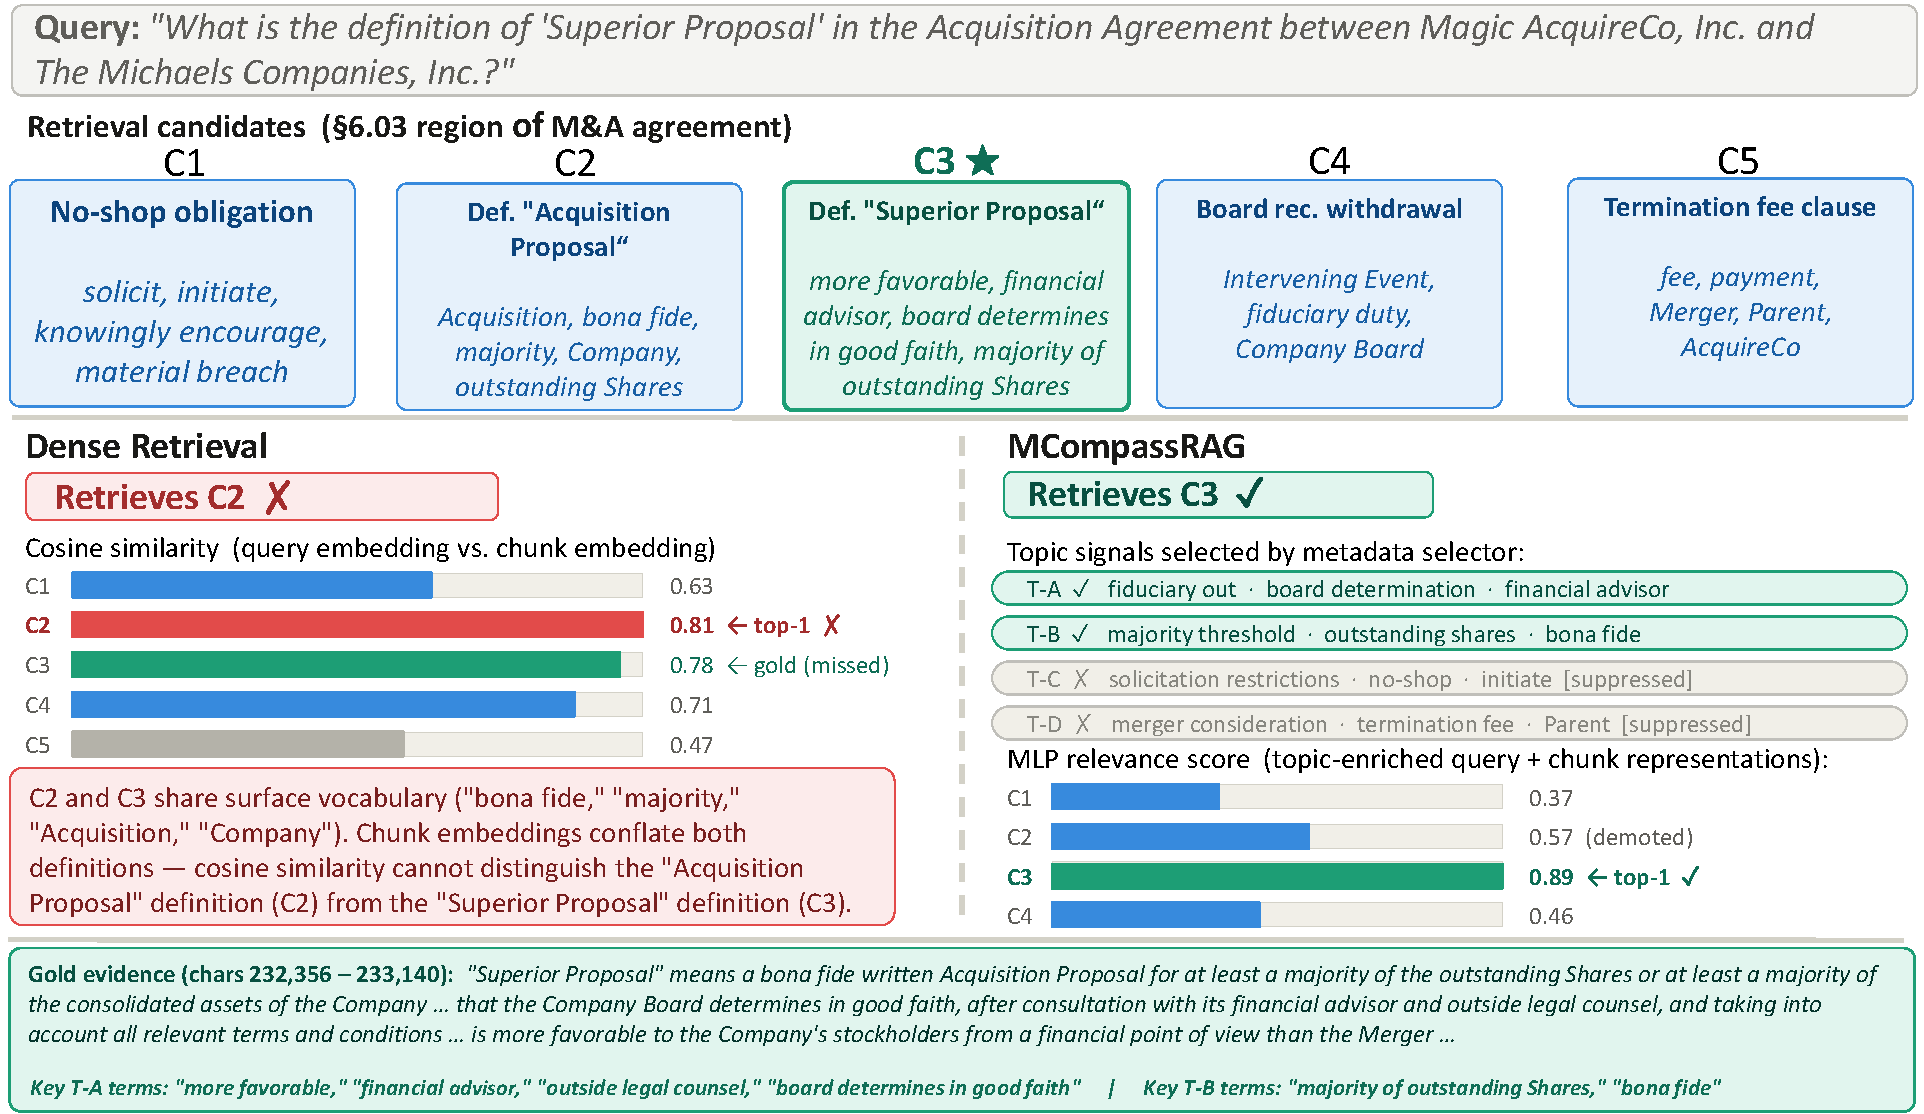
\includegraphics[width=\linewidth]{figures/CompassRAG_qualitative_comparison}
  \caption{Qualitative retrieval comparison on LegalBench-RAG for a query about the definition of \textit{Superior Proposal} in an M\&A acquisition agreement. \textbf{Top}: five retrieval candidates from the \S6.03 region; the gold chunk (C3, teal border) competes against four topically adjacent clauses sharing substantial surface vocabulary. \textbf{Bottom left}: dense retrieval ranks C2 (\textit{Acquisition Proposal} definition) above C3 due to overlapping tokens, missing the gold chunk at rank 1. \textbf{Bottom right}: \name{} activates topic signals T-A (fiduciary out / board determination) and T-B (majority threshold), suppresses T-C and T-D, and promotes C3 to rank 1 via the MLP scorer (0.89 vs.\ 0.57 for C2).}
  \label{fig:qualitative}
\end{figure*}

We present two qualitative examples to illustrate how \name{} resolves retrieval failures that dense similarity cannot handle: a definitional ambiguity case from LegalBench-RAG and an embedding-space analysis from Dragonball Finance.

\subsection{LegalBench-RAG: definitional ambiguity in M\&A agreements.} 
Figure~\ref{fig:qualitative} illustrates a concrete retrieval example from LegalBench-RAG that exposes the core failure mode of dense retrieval and how \name{} resolves it. The query asks for the definition of \textit{Superior Proposal} in an M\&A acquisition agreement whose \S6.03 region contains several topically adjacent clauses: a no-shop obligation (C1), the definition of \textit{Acquisition Proposal} (C2), a board recommendation withdrawal clause (C4), and a termination fee clause (C5). Dense retrieval assigns the highest cosine similarity to C2 (0.81) rather than the gold chunk C3 (0.78), ranking the wrong definition first. The failure arises because C2 and C3 share substantial surface vocabulary (``bona fide,'' ``majority,'' ``Acquisition,'' ``outstanding Shares''), causing their embeddings to occupy nearby positions in the retriever space. Cosine similarity cannot identify which latent topic of a chunk matches the query, nor distinguish a clause that \textit{defines} what counts as an acquisition proposal from one that \textit{evaluates} whether a proposal is superior.

\name{} recovers the gold chunk by activating two topic signals identified by the metadata selector as compatible with the query embedding: T-A, capturing the fiduciary-out and board determination frame (``more favorable,'' ``financial advisor,'' ``board determines in good faith''), and T-B, capturing the majority threshold frame (``majority of outstanding Shares,'' ``bona fide written Acquisition Proposal''). The selector simultaneously suppresses signals associated with solicitation restrictions (T-C) and merger consideration (T-D), which are prominent in the neighboring chunks but orthogonal to the query's information need. The abstraction module pools T-A and T-B into a compact query-side topic vector aligned with C3's own topic representation, and the MLP classifier assigns C3 a relevance score of 0.89 versus 0.57 for C2, promoting the correct definition to rank 1 without any inference-time LLM call. This disambiguation was learned through the teacher--student asymmetry in Section~\ref{sec:training}: the LLM teacher, given the expanded query framing the information need in terms of board determination and financial-advisor consultation, labels C3 as relevant and C2 as not, training the student to recover the same judgment through topic metadata alone.

\subsection{Dragonball Finance: topic-guided separation in embedding space.}
Figure~\ref{fig:tsne} visualizes the effect of topic enrichment on a Dragonball Finance example in which the query asks for a summary of Sparkling Clean Housekeeping Services' sustainability and social responsibility efforts in 2019. The eight retrieval candidates span the full thematic range of the company's corporate governance report: board composition (C1), executive remuneration (C2), risk management (C3), financial highlights (C4), shareholder structure (C5), internal audit (C6), and two surface-overlap distractors whose vocabulary partially overlaps with the gold chunk: a compliance and anti-corruption clause (C7, which shares the phrase ``corporate citizenship'') and a strategic outlook statement (C8, which shares ``long-term value creation'').

In the raw embedding space (Figure~\ref{fig:tsne}a), the query and the gold CSR chunk are already relatively proximate, yet several hard negatives remain in the same neighbourhood, reflecting the broad semantic overlap that coarse governance-report language introduces. After topic enrichment (Figure~\ref{fig:tsne}b), the query--gold alignment tightens substantially: the metadata selector activates the CSR topic centroid for the query and the gold chunk's own topic distribution loads on the same signal, pulling the two representations into close alignment while the hard negatives, whose dominant topic vectors correspond to governance, finance, and risk, drift away. The surface-overlap distractors C7 and C8 are particularly informative: despite sharing specific phrases with the gold chunk, their topic distributions do not load on the CSR centroid and therefore receive lower relevance scores from the MLP classifier, confirming that \name{}'s disambiguation operates at the level of latent topic structure rather than lexical overlap.

\begin{figure*}[t]
  \centering
  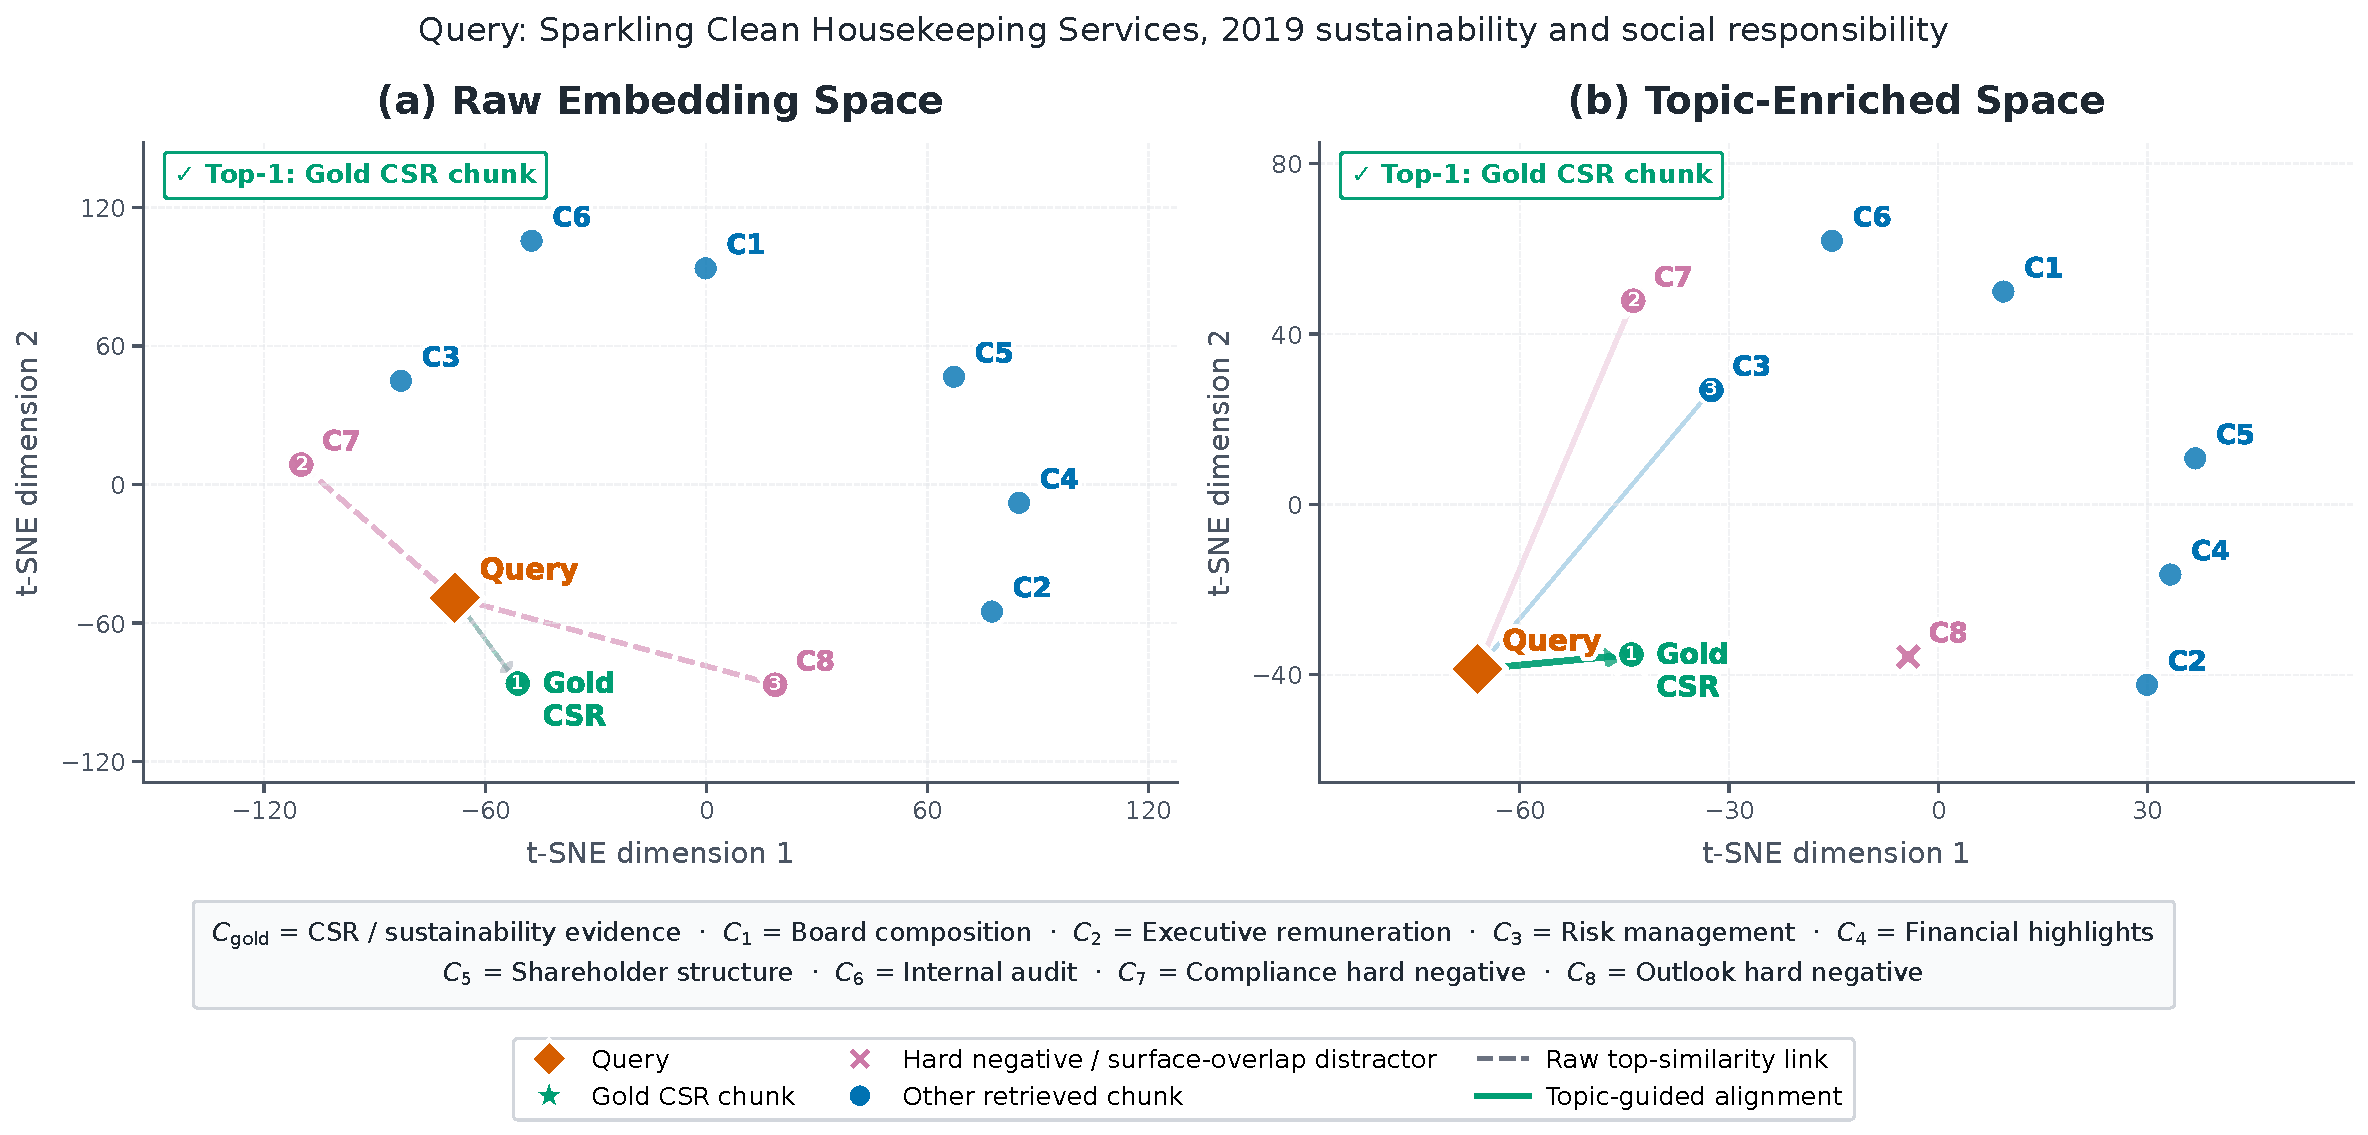
\includegraphics[width=\linewidth]{figures/tsne_qualitative_new.pdf}
  \caption{t-SNE visualization of chunk embeddings for a Dragonball Finance query on Sparkling Clean Housekeeping Services' 2019 sustainability efforts. Chunks cover eight aspects of the corporate governance report: board composition (C1), executive remuneration (C2), risk management (C3), financial highlights (C4), shareholde structure (C5), internal audit (C6), compliance and anti-corruption (C7), and strategic outlook (C8); C7 and C8 are surface-overlap distractors that share phrases with the gold CSR chunk. \textbf{(a) Raw embedding space}: the query and gold chunk are proximate but several hard negatives occupy the same neighbourhood. \textbf{(b) Topic-enriched space}: topic enrichment tightens the query--gold alignment while pushing all hard negatives, including the surface-overlap distractors C7 and C8, away from the query.}
  \label{fig:tsne}
\end{figure*}